% Author : Bhishan Poudel
% Date   : Apr 11, 2016
% Ref    : https://en.wikibooks.org/wiki/LaTeX/Labels_and_Cross-referencing


\documentclass{article}
\usepackage[english]{babel}
\usepackage{graphicx}
\usepackage[letterpaper]{geometry}
\geometry{top=1.0in, bottom=1.0in, left=1.5in, right=1.0in}
\usepackage{flafter} % make sure figures do not appear before their text
\usepackage{sidecap} % use side captions for floats
\usepackage{subfig} % subfloats

%for referencing
\usepackage{amsmath} % for \eqref{}
\usepackage{fancyref}
%\usepackage{showkeys}
\usepackage{hyperref} % gives hyperlink of contents
\usepackage[hypcap]{caption} % to use with hypref

\title{}
\author{Bhishan Poudel}
\date{\today}
\author{Bhishan Poudel}
\begin{document}

\title{}
\tableofcontents
\listoffigures

\section{Referencing a figure}
Referencing tags: \\
ch: 	chapter \\
sec: 	section\\
subsec: 	subsection\\
fig: 	figure\\
tab: 	table\\
eq: 	equation\\
lst: 	code listing\\
itm: 	enumerated list item\\
alg: 	algorithm\\
app: 	appendix subsection\\

%%%%%%%%%% figure environment start %%%%%%%%%%%%%%%%%
\begin{figure}[ht!]
\centering
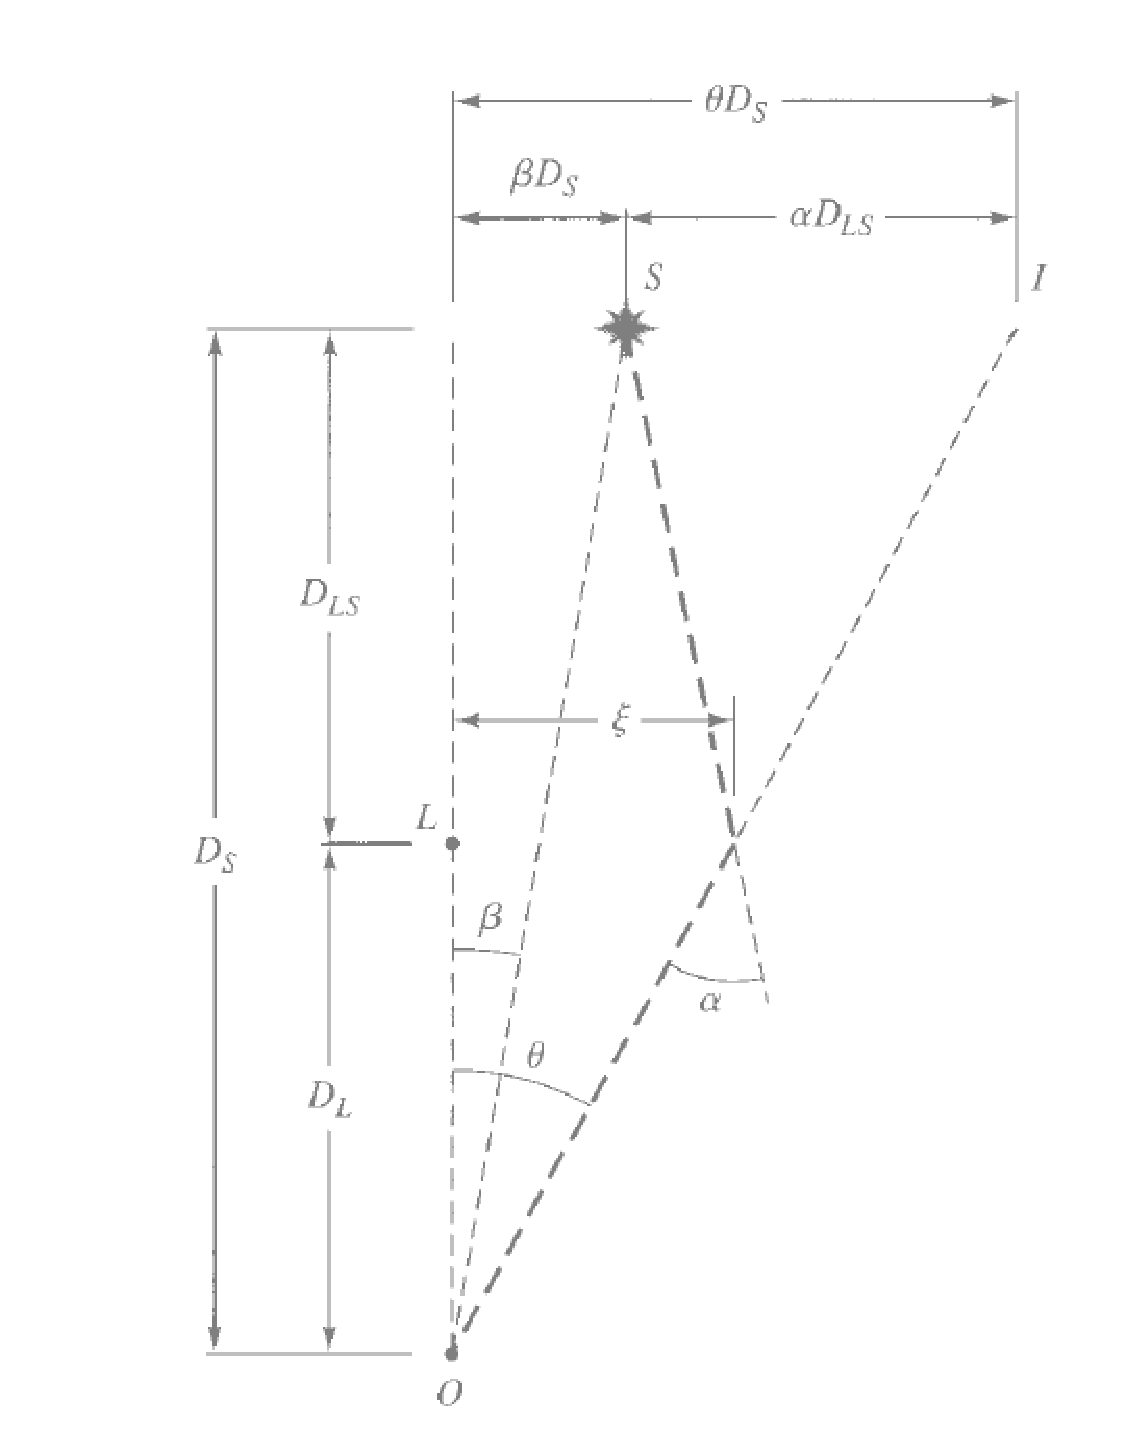
\includegraphics[scale = 0.5]{images/fig1.eps}
\caption{Deflection of light by a spherical massive body}
\label{fig:fig1} % this is good habit of prefixing fig: for figure
\end{figure}
%%%%%%%%%% figure environment end %%%%%%%%%%%%%%%%%
The command label must appear after (or inside) caption. Otherwise, it will pick up the current section or list number instead of what you intended.

See figure ~\ref{fig:fig1} on page~\pageref{fig:fig1}.\\
You have to compile your document twice to see the proper output. If you compile it only once, LaTeX will use the older information it collected in previous compilations.

\section{Formulae}
\label{sec:Formulae}

Here is an example showing how to reference formulae:

\begin{equation} \label{eq:solve}
x^2 - 5 x + 6 = 0
\end{equation}

\begin{equation}
x_1 = \frac{5 + \sqrt{25 - 4 \times 6}}{2} = 3
\end{equation}

\begin{equation}
x_2 = \frac{5 - \sqrt{25 - 4 \times 6}}{2} = 2
\end{equation}

and so we have solved equation~\ref{eq:solve}.

\section{Greetings}
\label{sec:greetings}

Hello!

\section{Referencing}

I greeted in section~\ref{sec:greetings}.
You could place the label anywhere in the section; however, in order to avoid confusion, it is better to place it immediately after the beginning of the section. Note how the marker starts with sec:, as suggested before. The label is then referenced in a different section. The tilde (\textasciitilde) indicates a non-breaking space.

\section{The hyperref package}
\subsection{autoref}

This is hyperlink to \autoref{sec:Formulae} created using hyperref package and autoref command.\\

The hyperref package introduces another useful command; \textbf{autoref{}}. This command creates a reference with additional text corresponding to the target's type, all of which will be a hyperlink. For example, the command \textbf{autoref{sec:intro}} would create a hyperlink to the \label{sec:intro} command, wherever it is. Assuming that this label is pointing to a section, the hyperlink would contain the text "section 3.4", or similar (the full list of default names can be found here). Note that, while there's an \textbf{autoref* }command that produces an unlinked prefix (useful if the label is on the same page as the reference), no alternative \textbf{Autoref} command is defined to produce capitalized versions (useful, for instance, when starting sentences); but since the capitalization of autoref names was chosen by the package author, you can customize the prefixed text by redefining \textbf{typeautorefname} to the prefix you want, as in:

\textbf{def~~\sectionautorefname{Section}}

This renaming trick can, of course, be used for other purposes as well.

    If you would like a hyperlink reference, but do not want the predefined text that\textbf{ autoref{}} provides, you can do this with a command such as \textbf{hyperref[sec:intro]{Appendix~\ref*{sec:intro}}.} Note that you can disable the creation of hyperlinks in hyperref, and just use these commands for automatic text.

    Keep in mind that the \textbf{label} must be placed inside an environment with a counter, such as a table or a figure. Otherwise, not only the number will refer to the current section, as mentioned above, but the name will refer to the previous environment with a counter. For example, if you put a label after closing a figure, the label will still say "figure n", on which n is the current section number.

\subsection{nameref}

The hyperref package also automatically includes the nameref package, and a similarly named command. It is similar to \textbf{autoref{}}, but inserts text corresponding to the section name, for example.

\section{MyFirstSection} \label{sec:marker}
\section{MySecondSection}
In section~\nameref{sec:marker} we defined...

\section{Displaying reference marker on output pdf}
If you want to be able to see the markers you are using in the output document as well, 
you can use the showkeys package; this can be very useful while developing your document.



\end{document}